\documentclass[12pt]{article}
\usepackage[margin=1in]{geometry}
\usepackage{amsmath,amsthm,amssymb,amsfonts}
\usepackage{graphicx}
\usepackage{physics}
%\usepackage{halloweenmath}
\usepackage{setspace}
\usepackage[font=small,labelfont=bf]{caption}

\newcommand{\N}{\mathbb{N}}
\newcommand{\Z}{\mathbb{Z}}

\newenvironment{part}[2][Part]{\begin{trivlist}
\item[\hskip \labelsep {\bfseries #1}\hskip \labelsep {\bfseries #2.}]}{\end{trivlist}}
%If you want to title your bold things something different just make another thing exactly like this but replace "problem" with the name of the thing you want, like theorem or lemma or whatever

\graphicspath{ {./} }

\begin{document}

\title{\textbf{ASTR 522: Lab 2}}
\author{Jonas Powell}
\maketitle


%\twocolumn
\begin{onehalfspacing}


\iffalse
For part 1, describe the methodology you used to determine most probable astronomical source.
\fi
\raggedright{\textbf{\Large Part 4}}\\

For Part 1, I implemented the cost function:

\begin{align*}
  C &= c_1 \, \frac{V}{V_{\text{max}}} + (c_2 = 1 - c1) \frac{d}{d_{\text{max}}} \\
\end{align*}

where $V$ was the source's V-band magnitude (given in the results of a query of the Vizier V/50 bright star catalog accessed through astroquery), and $d$ was the source's Pythagorean distance, in decimal degrees, each scaled by the maximum value of each quantity given in the query's results (since more than one source is usually returned). This normalization, while not totally necessary, does guarantee that $[\frac{V}{V_{\text{max}}}, c_2 \frac{d}{d_{\text{max}}}] \leq 1$, which allows us to treat $c_1$ and $c_2$ as traditionally weights and tune the influence of each element as we see fit. For this problem, I just set $c_1 = c_2 = 0.5$ for simplicity's sake, and because I couldn't come up with a good reason to prefer proximity to the requested sky coordinates over brightness; each should obviously play a role but considering how those roles relate is deserving of further thought.




\iffalse
For part 2, how does the uncertainty in your geographic position compare with the uncertainty in astronomical coordinates from the previous problem?

\fi
\raggedright{\textbf{\Large Part 3}}\\
Significantly! My method for determining geographic location is able to 




%% FIGURES
\newpage


%\iffalse
\begin{figure}
    \centering
    \begin{minipage}{0.48\textwidth}
        \centering
        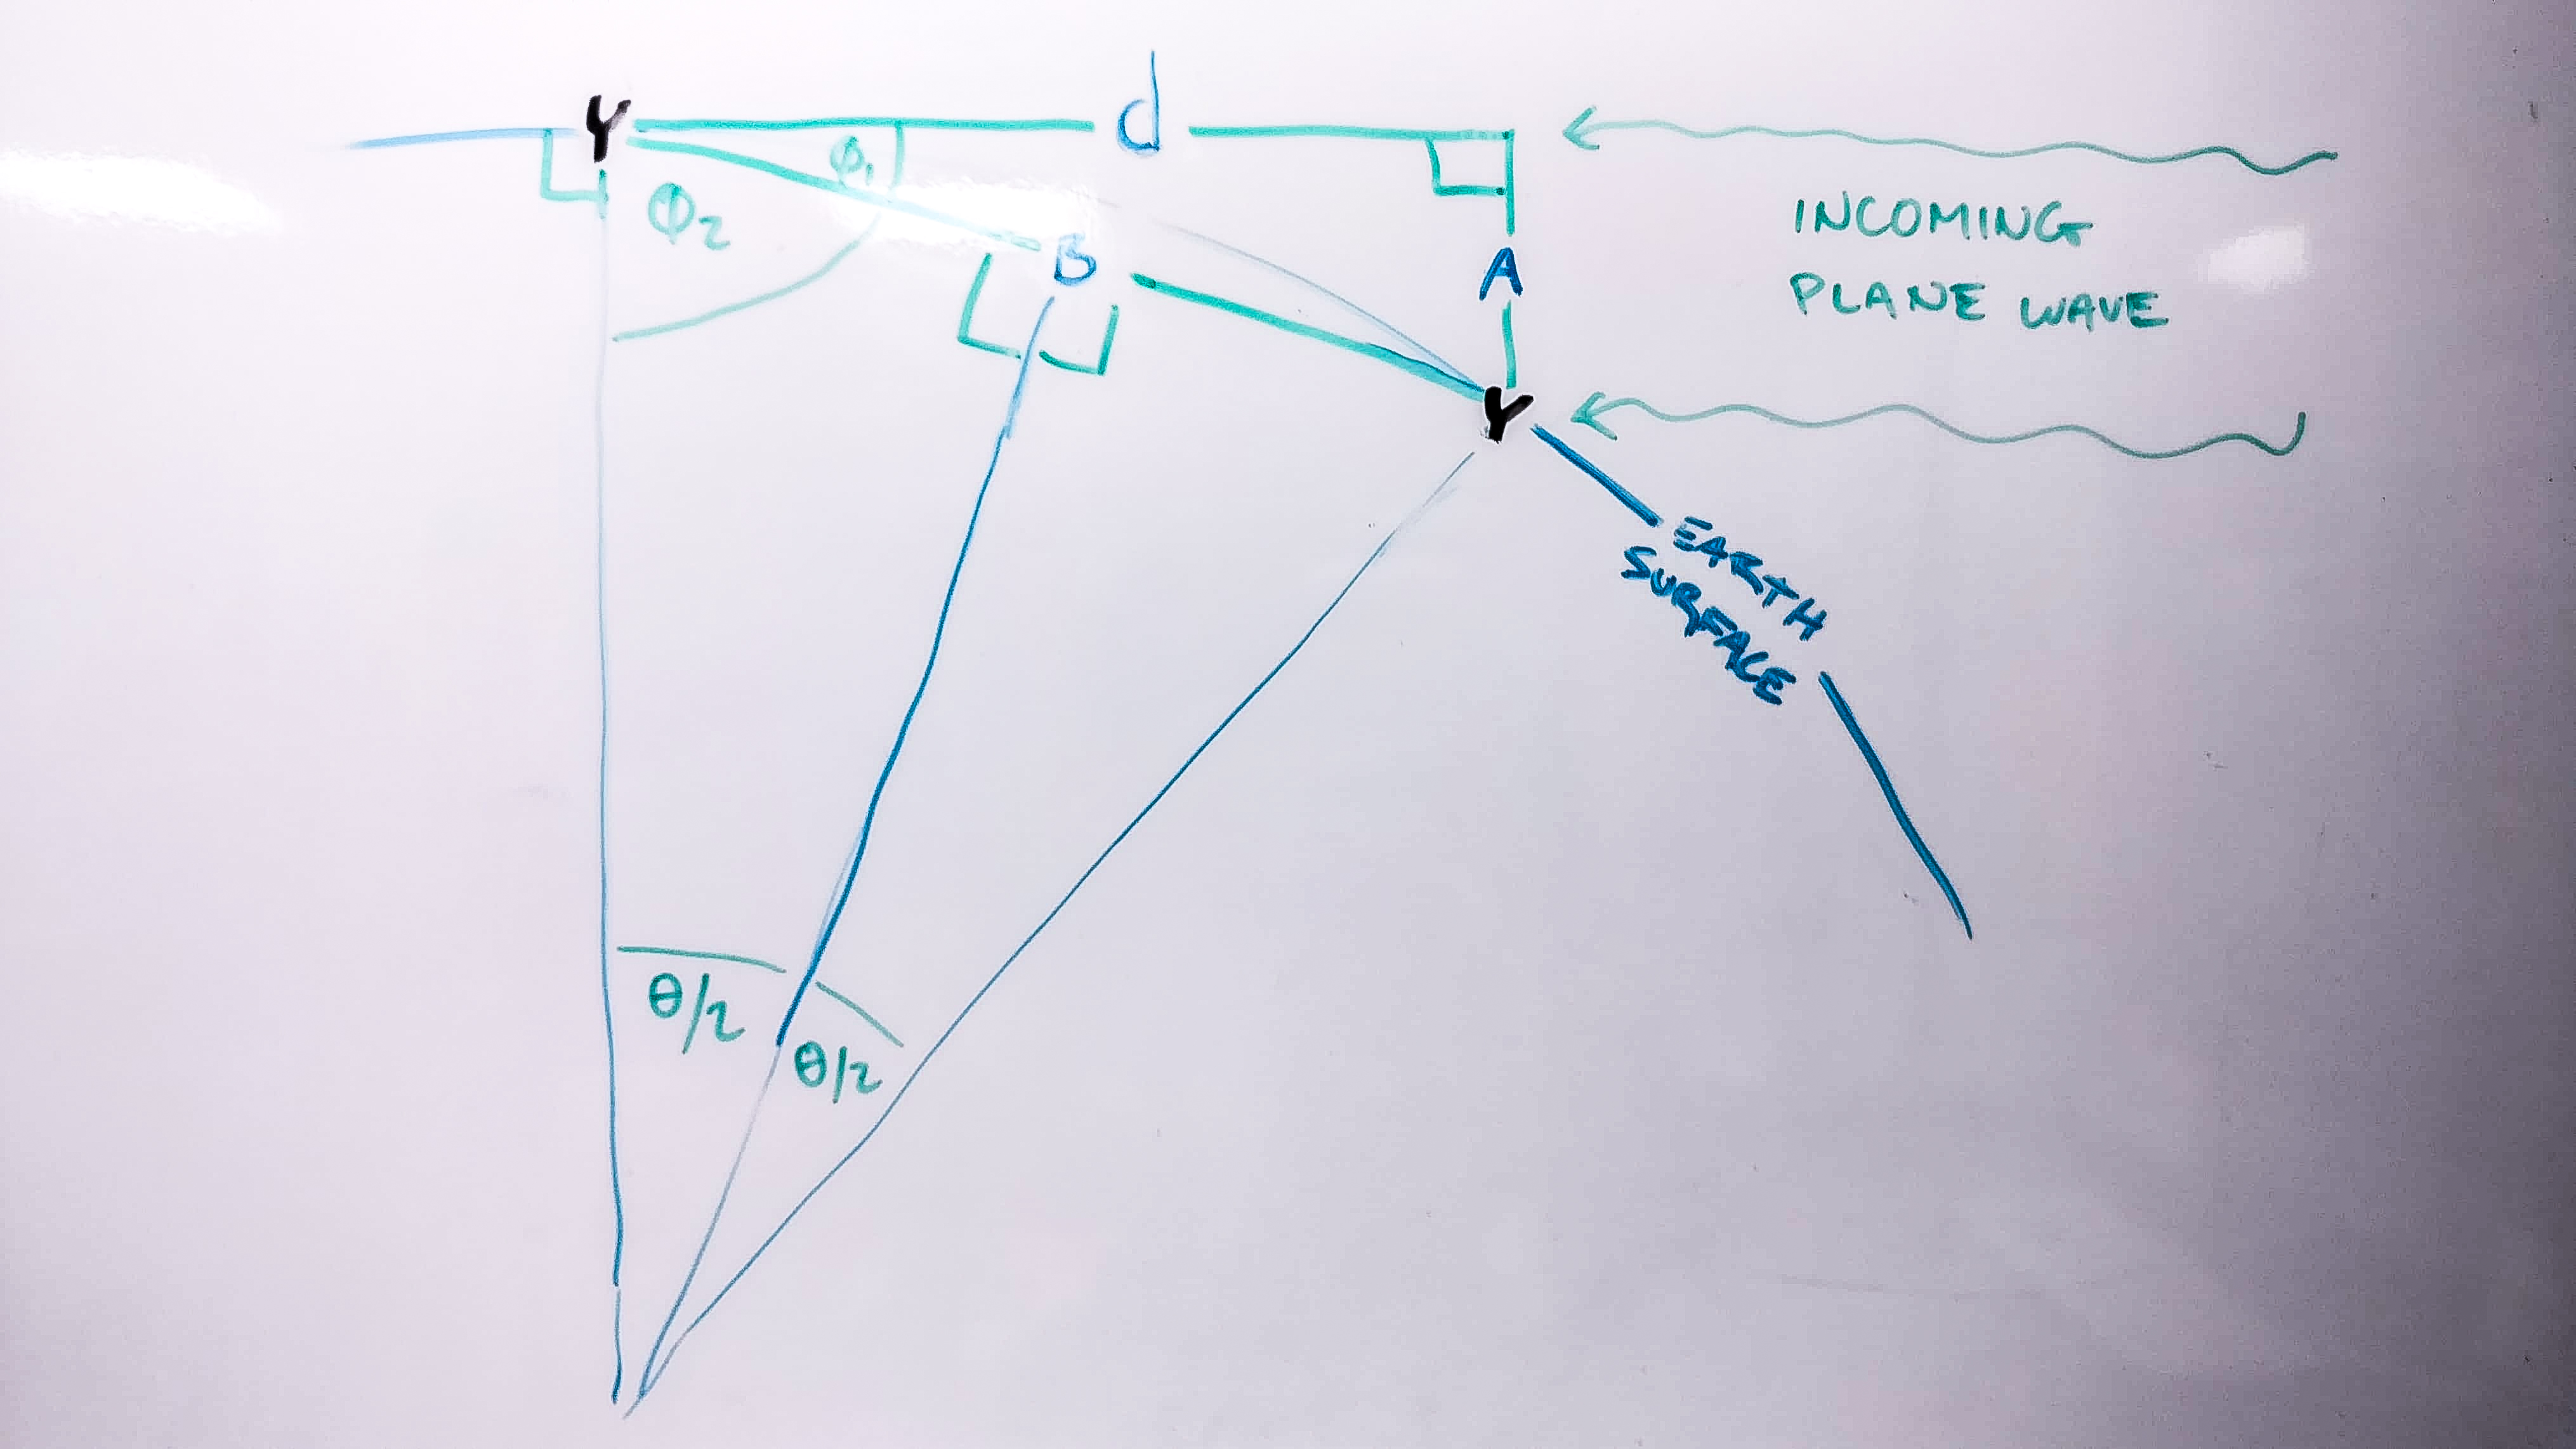
\includegraphics[width=0.95\textwidth]{prob1b} % first figure itself
        \caption{Signal from a source at one source's horizon results in this geometric event, from which we can find difference in path length for signal reaching each dish.}
    \end{minipage}\hfill
    \begin{minipage}{0.48\textwidth}
        \centering
        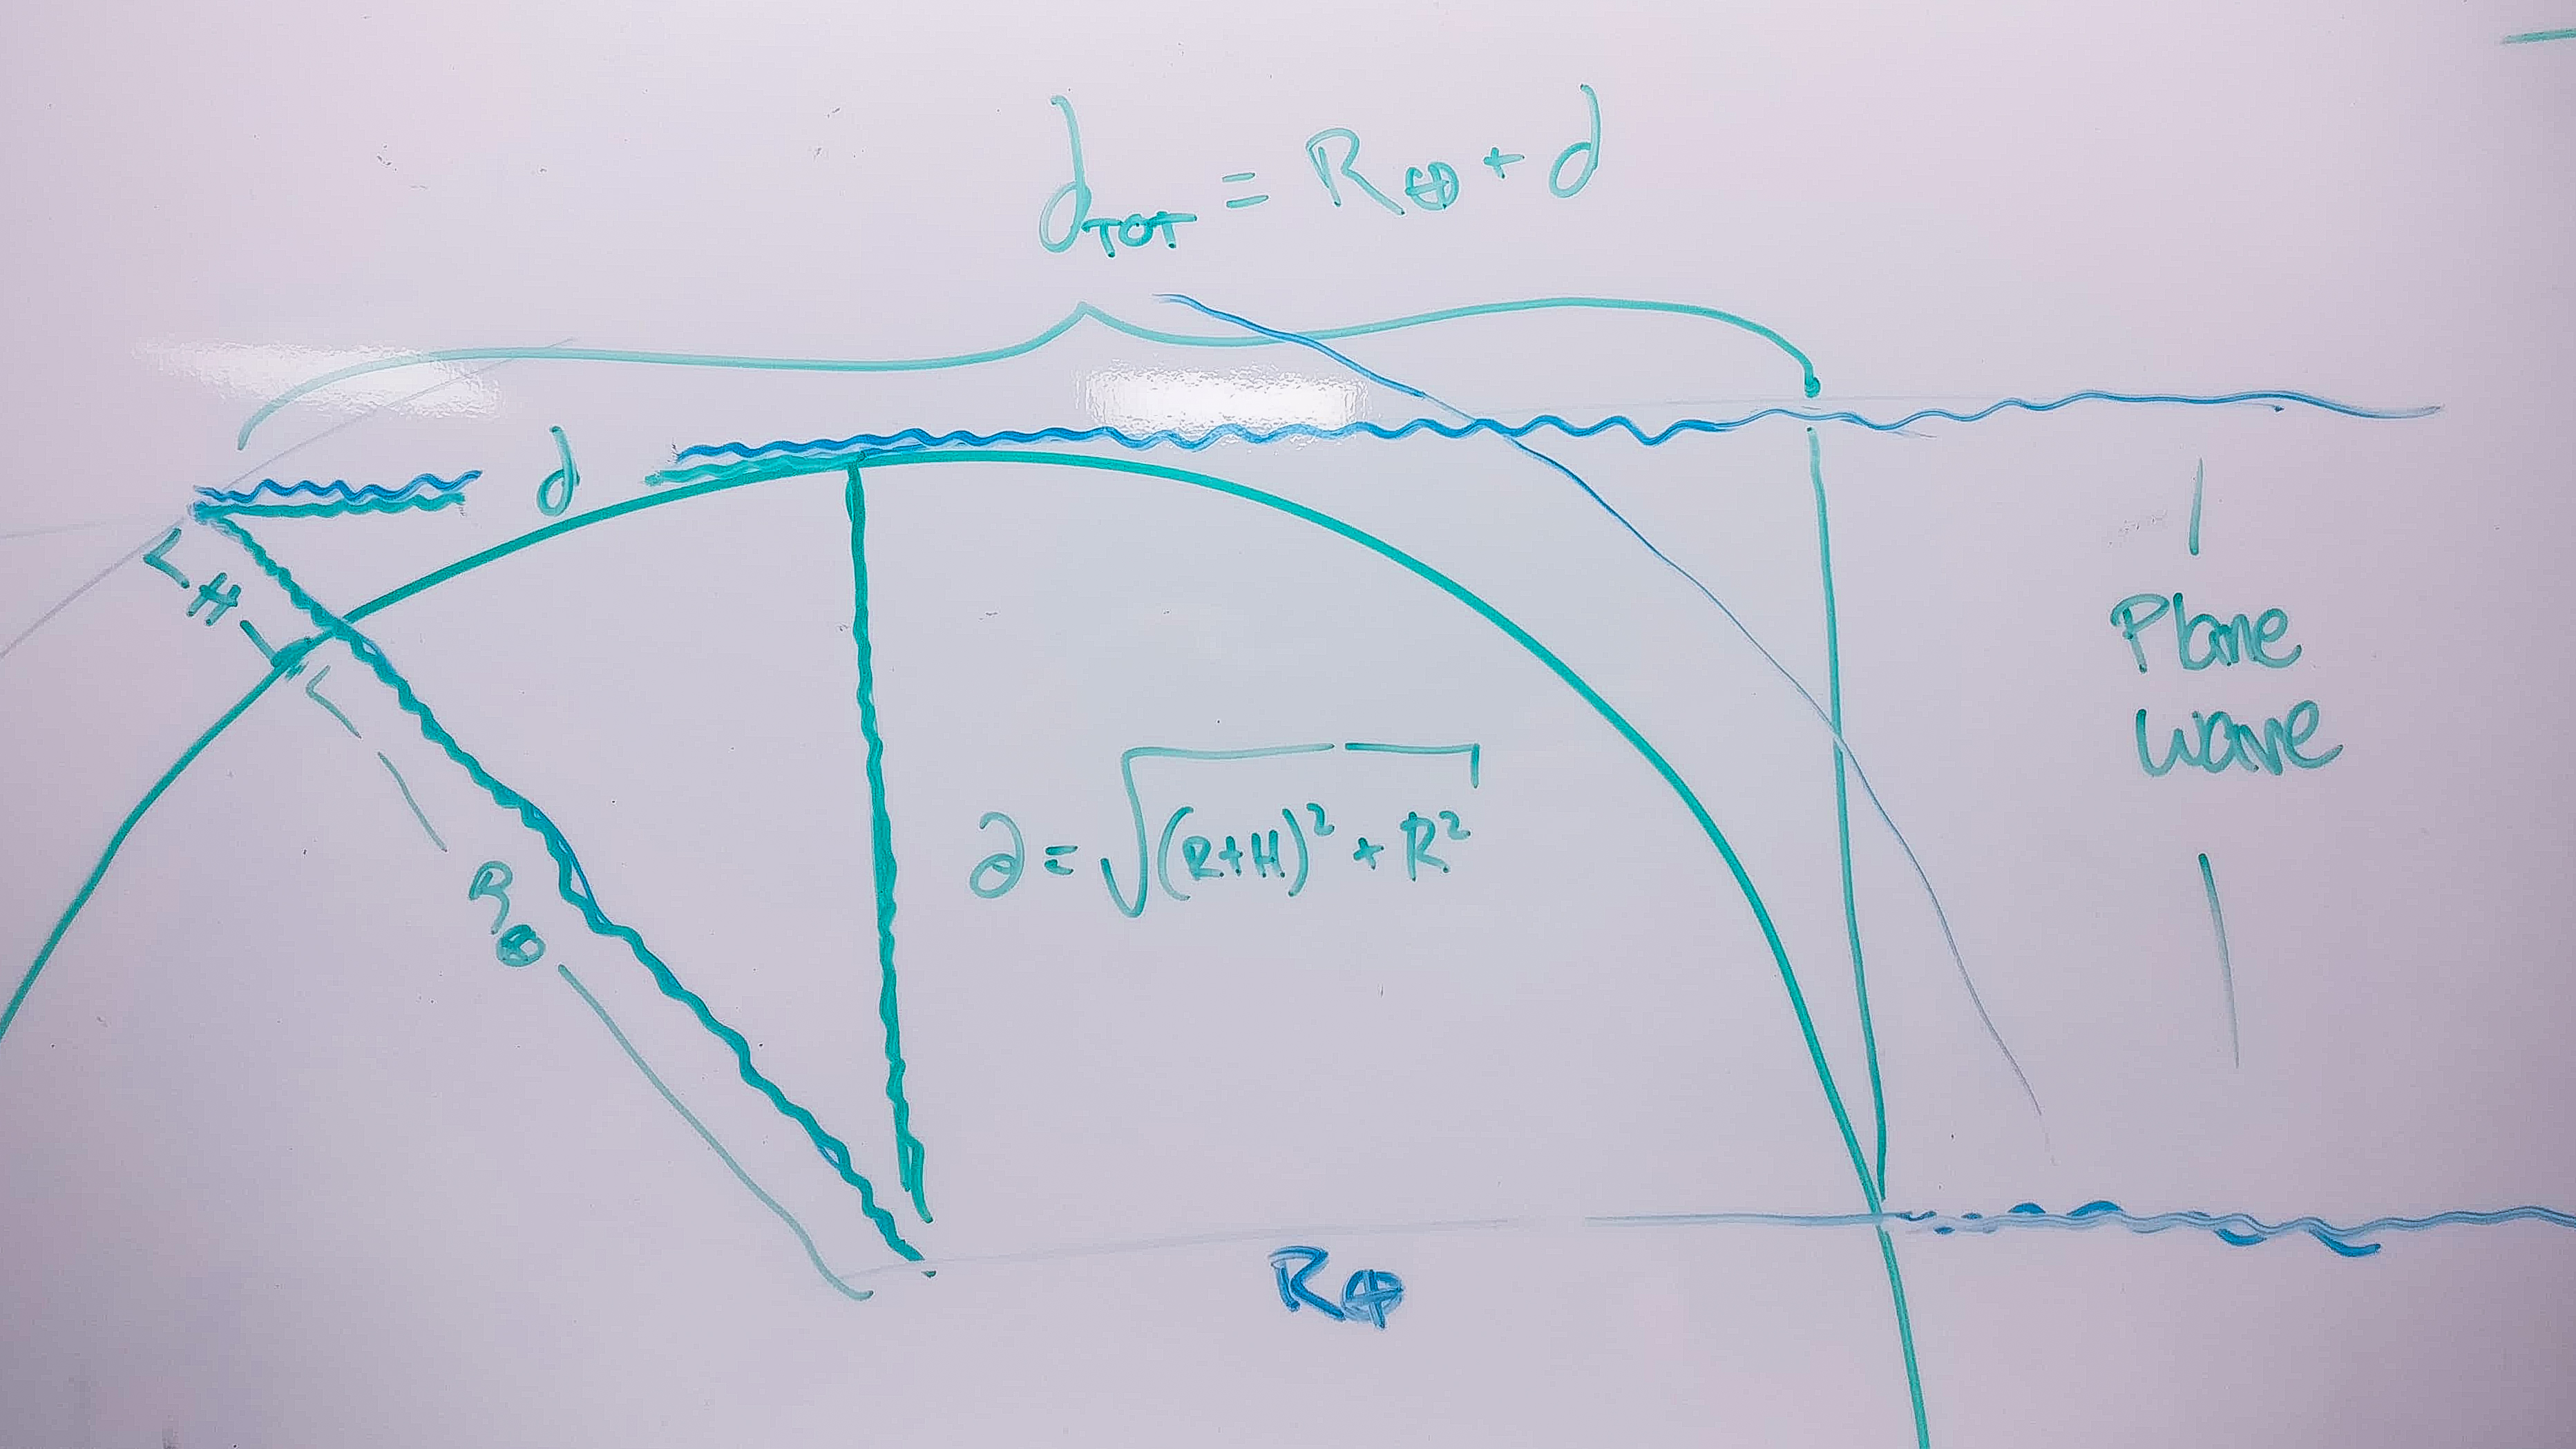
\includegraphics[width=0.95\textwidth]{prob2b} % second figure itself
        \caption{Signal from a source at one source's horizon results in this geometric event, from which we can find difference in path length for signal reaching each dish.}
    \end{minipage}
\end{figure}






\bigskip
\bigskip
\end{onehalfspacing}

\end{document}
